\chapter{Architektur}
\label{ch:Architektur}
Unsere Implementierung ist in dem Plugin tools.vitruv.applications.pcmjava.integrationFromGit. Die Tests befinden sich in dem Plugin\\ tools.vitruv.applications.pcmjava.integrationFromGit.test. Die unvollständigen Klassendiagramme für die beiden Plugins sind in den Abbildungen \ref{fig:integrationFromGit} und \ref{fig:integrationFromGit_test} dargestellt.

\begin{figure}[h]
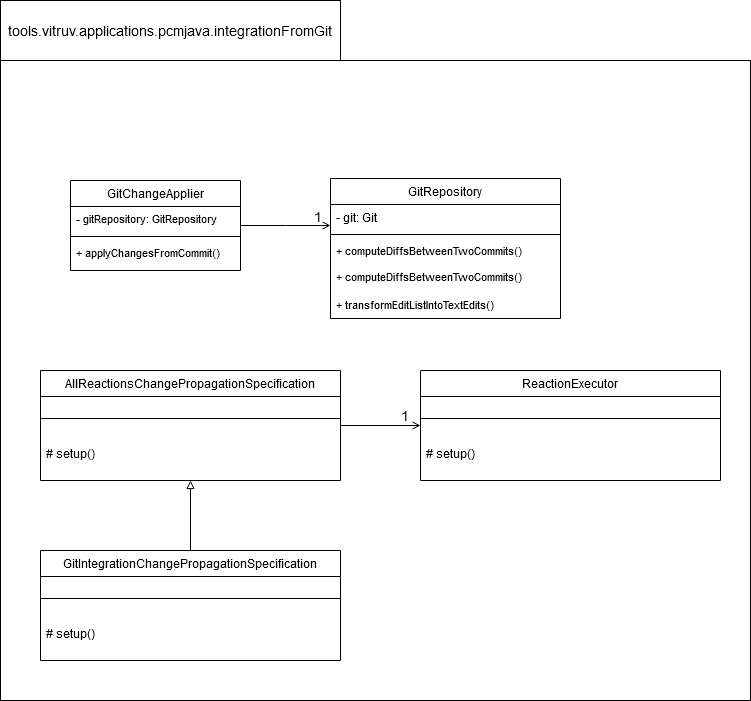
\includegraphics[width=\textwidth]{pictures/integrationFromGit_diagram.png}
\caption{Klassendiagram für das Plugin tools.vitruv.applications.pcmjava.integrationFromGit. Das Klassendiagramm ist unvollständig und dient nur einer Darstellung der einzelnen Klassen, Methoden und Variablen.}
\label{fig:integrationFromGit}
\end{figure}

\begin{figure}[h]
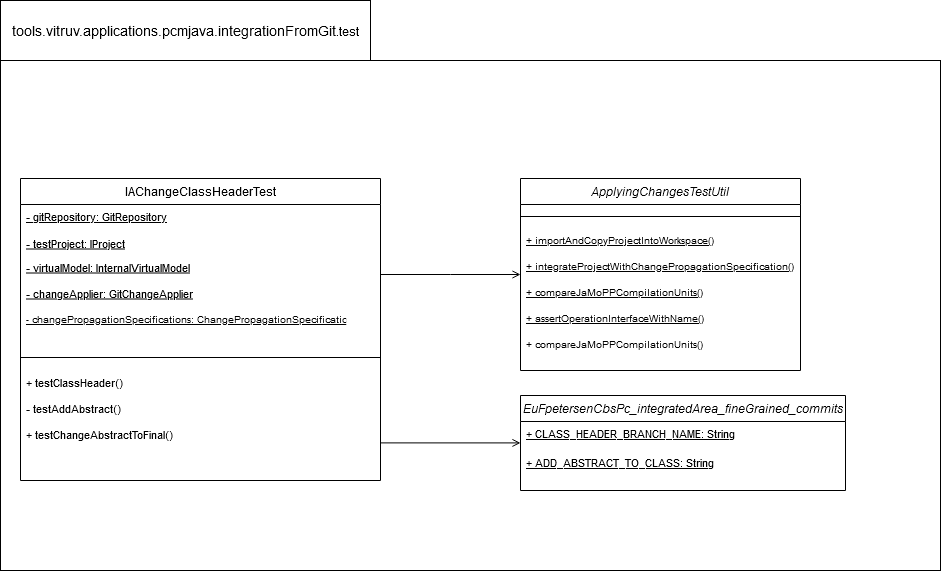
\includegraphics[width=\textwidth]{pictures/integrationFromGitTest_diagram.png}
\caption{Klassendiagram für das Plugin tools.vitruv.applications.pcmjava.integrationFromGit.test. Das Klassendiagramm ist unvollständig und dient nur einer Darstellung der einzelnen Klassen, Methoden und Variablen.}
\label{fig:integrationFromGit_test}
\end{figure}

\section{Plugin tools.vitruv.applications.pcmjava.integrationFromGit}

Die Klasse GitChangeApplier wendet extrahierte Änderungen auf die Code-Modelle an. Die Hauptmethode applyChangesFromCommit nimmt als Parameter zwei Commits, zwischen denen Änderungen ausgerechnet werden müssen, sowie ein JDT-Modell von einem Java-Projekt. Die Methode ermittelt Änderungen, klassifiziert sie und ruft eine passende Routine auf. Zum Beispiel, für eine als 'ADD' klassifizierte Änderung wird die Methode addElementToProject aufgerufen. Nach einer erfolgreichen Ausführung sind die Änderungen auf das JDT-Modell von dem Java-Projekt angewandt. Falls dieses Projekt in Vitruvius integriert ist, werden auch die JaMoPP-Modelle in VSUM automatisch angepasst und gegebenenfalls auch die korrespondierenden PCM-Modelle.
\\ 
Anders als in dem GitChangeReplay-Tool \footnote{GitChangeReplay-Tool: https://github.com/vitruv-tools/GitChangeReplay} werden in unserer Implementierung die aus einem Commit extrahierten Änderungen nicht in atomare Änderungen zerlegt. Für unseren Zweck ist es nicht notwendig. Darüber hinaus würde das die Performance unserer Implementierung negativ beeinträchtigen.
\\
Änderungen an den JaMoPP-Modellen in VSUM werden von dem Monitor detektiert. Anschließend werden die entsprechenden Listener benachrichtigt. Dieser Mechanismus ermöglicht eine Aktualisierung von den korrespondierenden Performance-Modellen. Als Performance-Modelle haben wir die Palladio Component Models (PCM) benutzt. Um die Performance-Modelle automatisch anpassen zu können, muss eine Change Propagation Specification (CPS) und Change Propagation Rules (CPR) definiert werden. Unsere CPS ist in der Klasse GitIntegrationChangePropagationSpecification definiert. Die CPR haben wir in der Reaction-Sprache definiert. Sie befinden sich in den Dateien PackageAndClassifiers.reactions und ClassifierBody.reactions. Die meisten CPR haben wir aus den folgenden Projekten übernommen und angepasst:

\begin{itemize}
\item \begin{scriptsize}
tools.vitruv.applications.pcmjava.linkingintegration.change2command.internal.response.PackageMappingIntegration.reactions\end{scriptsize}
\item tools.vitruv.applications.pcmjava.pojotransformations.java2pcm
\end{itemize}

Die CPR für die Änderungen innerhalb der Methoden haben wir unverändert gelassen. Sie stammen aus dem folgenden Projekt:
\begin{itemize}
\item \begin{scriptsize}tools.vitruv.applications.pcmjava.seffstatements.pojotransformations.Java2PcmPackageMappingMethodBodyChangePreprocessor.xtend
\end{scriptsize}\end{itemize}

Außerdem haben wir auch neue CPR definiert. Zum Beispiel eine Reaktion auf löschen einer Klasse und eines Packages. Die Anpassungen in den bereits existierenden CPR waren notwendig, weil sie für unsere Case-Study nicht (korrekt) funktioniert haben. Ein Grund dafür war, dass die ursprünglichen CPR nicht für die integrierten Projekte gedacht sind, sondern für die Projekte, die von Anfang an mit Vitruvius entwickelt wurden. Zum Beispiel, wenn ein neues Package erstellt wurde, wurden automatisch  Subpackages 'datatypes' und 'contracts' erstellt. Das hat aber zu Inkonsistenzen zwischen der Projektstruktur in dem Git Repository und der in Vitruvius geführt, weil in Git Repository keine Subpackages 'datatypes' und 'contracts' existieren.

\section{Plugin tools.vitruv.applications.pcmjava.integrationFromGit.test}

Die Tests haben wir in zwei Packages unterteilt:

\begin{itemize}
\item tools.vitruv.applications.pcmjava.integrationFromGit.test.integratedArea
\item tools.vitruv.applications.pcmjava.integrationFromGit.test.nonIntegratedArea
\end{itemize}

Die Tests in tools.vitruv.applications.pcmjava.integrationFromGit.test.integratedArea simulieren Änderungen auf den Teilen des Projekts, die bereits vor der Integration in Vitruv existiert haben und als einen integrierten Bereich zählen. Was als ein integrierter Bereich zählt ist projektspezifisch. In unserem Test-Projekt gelten alle Packages innerhalb des source-Packages als integrierten Bereich. Mehr Details über integrierte und nicht integrierte Bereiche können in \cite{langhammer2017} gefunden werden. Die Tests in\\ tools.vitruv.applications.pcmjava.integrationFromGit.test.integratedArea simulieren Änderungen auf den Teilen des Projekts, die vor der Integration in Vitruv noch nicht existiert haben. Außerdem finden diese Änderungen in einem Bereich statt, der als nicht integrierten Bereich zählt. In unserem Test-Projekt zählt ein neues Package innerhalb des source-Packages als ein nicht integrierter Bereich. Das neue Package darf nicht in die anderen schon existierenden Subpackages verschachtelt sein. Sonst würde es als ein integrierter Bereich erkannt.
\\
In unseren Tests wollten wir zeigen, dass die von uns angepassten Change Propagation Rules (CPR) sich gleich verhalten ungeachtet darauf, ob Änderungen in einem integrierten oder nicht integrierten Bereich stattgefunden haben. In der Zukunft sollte diese Unterscheidung komplett irrelevant sein, weil der CIPM-Ansatz \cite{mazkatli2018} auf den Java-Projekten mit beliebigen Strukturen anwendbar sein soll.
\\
In dem Package tools.vitruv.applications.pcmjava.integrationFromGit.test.commits sind die Namen von den Git-Branches und Commit-Hashes für alle Tests gespeichert.
\\
In dem Ordner tools.vitruv.applications.pcmjava.integrationFromGit.test/testProjects ist unser Test-Projekt gespeichert.
\\
In der Klasse ApplyingChangesTestUtil.java sind die Hilfsmethoden für alle Tests enthalten. Die meisten Methoden sind statisch und können deshalb auch in den anderen Projekten benutzt werden.
\\
Jeder Test überprüft die Korrektheit unserer Implementierung für einen bestimmten Änderungstypen. Zum Beispiel der Test IAChangeClassHeaderTest.java simuliert Änderungen eines Klassenkopfes. Das Präfix 'IA' steht für Integrated Area und 'NIA' für Non-Integrated Area. Alle Tests haben eine ähnliche Struktur:
\\
1. Vorbereitung (setUpBeforeClass-Methode):
\\
Zuerst wird ein Projekt in das aktuelle Workspace kopiert und ein JDT-Modell davon erstellt (IProject testProject). Ebenso wird dieses Projekt mit seinem Git-Repository in das Workspace kopiert (in einen separaten Ordner namens 'clonedGitRepositories'). Die Objekte GitRepository und GitChangeApplier verweisen auf 'clonedGitRepositories'. Das erstellte JDT-Modell (IProject testProject) wird in Vitruvius integriert. Dabei entsteht ein Ordner 'vitruvius.meta' in dem Workspace, ein Monitor, der Änderungen zu den korrespondierenden Modellen propagiert, und ein InternalVirtualModel-Objekt. Das InternalVirtualModel-Objekt enthält unter anderem eine Referenz auf die 'vitruvius.meta'-Ordner und\\GitIntegrationChangePropagationSpecification-Objekt. Für die Tests in den nicht integrierten Bereichen werden auch nicht integrierte Bereiche vorbereitet (Packages, Klassen, Interfaces erstellt).
\\
2. Der eigentliche Test:
\\
Die Abbildung \ref{fig:method} zeigt einen Test für das Hinzufügen einer Klassenvariable in einer Klasse, die in einem integrierten Bereich liegt. Zuerst wird eine Änderung  aus einem Commit gelesen und auf das in Vitruvius integrierte Projekt angewandt (changeApplier.applyChangesFromCommit(...)) und das geänderte JDT-Modell gefunden (ICompilationUnit compUnitChanged). Als Referenzmodell wird das Git-Repository an dem gleichen Commit ausgecheckt und ein temporäres JDT-Modell von der gleichen (aber nicht der selben) Compilation Unit erstellt (gitRepository.checkoutFromCommitId(...) und ICompilationUnit compUnitFromGit). Anschließend werden die JaMoPP-Modelle für die beiden Compilation Units (compUnitChanged und compUnitFromGit) verglichen (ApplyingChangesTestUtil.compareJaMoPPCompilationUnits(...)). Das JaMoPP-Modell für compUnitFromGit wird neu erstellt während das JaMoPP-Modell für compUnitChanged wird aus InternalVirtualModel genommen. Als letztes wird es überprüft, ob ein PCM-Modell für die neu erstellte Klassenvariable existiert (ApplyingChangesTestUtil.assertFieldWithName(...)). Eine explizite Überprüfung der nötigen Korrespondenz ist nicht notwendig, weil sie implizit in der Methode ApplyingChangesTestUtil.assertFieldWithName(...) stattfindet.
\begin{figure}[h]
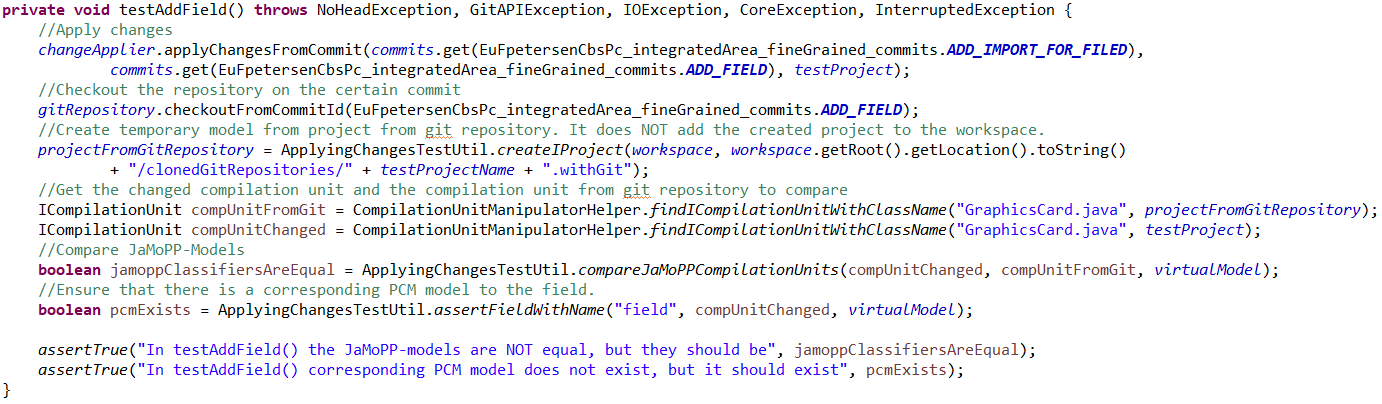
\includegraphics[width=\textwidth]{pictures/method_example.png}
\caption{Test für das Hinzufügen einer Klassenvariable in einer Klasse, die in einem integrierten Bereich liegt}
\label{fig:method}
\end{figure}